\documentclass{article}

% Language setting
\usepackage[english]{babel}

% Set page size and margins
\usepackage[letterpaper,top=2cm,bottom=2cm,left=3cm,right=3cm,marginparwidth=1.75cm]{geometry}

% Useful packages
\usepackage{amsmath}
\usepackage{graphicx}
\usepackage[colorlinks=true, allcolors=blue]{hyperref}
\usepackage{listings}
\lstset{language=C, basicstyle=\ttfamily\footnotesize, frame=single, breaklines=true}

\title{CPE 301 Embedded Systems Design Final Project}
\author{Aidan Swan, Nathan Saxe, Canon Leahy, & Nate Gomez}

\begin{document}
\maketitle
\section{Introduction}
This final project focuses on developing a swamp cooler using the Arduino 2560 microcontroller and sensors used from previous labs. The goal of this project was to create a functioning cooler which monitors water levels, stops and starts fans at a certain temperature, allows user control to adjust the angle of the vent, an on/off button, and a record of when the device is turned off or on. Using Arduino libraries and direct register manipulation allows for precise control and information to be displayed on the LCD. We used a real-time clock to monitor events and used the DHT11 for temperature and humidity readings. The system is continuously monitored and  the stepper motor allows for vent angling. Combining everything creates an optimized cooling process. 

\section{Equipment Used}
The following equipment and components were used in the project:
\begin{itemize}
    \item Arduino ATmega2560 microcontroller
    \item USB cable
    \item Breadboards
    \item LED
    \item Buttons
    \item LCD display
    \item Fan
    \item Stepper Motor
    \item Resistors
    \item DHT11 Temp / Humidity Sensor
    \item Water Detection Sensor
    \item Potentiometer
    \item Wires
    \item 9 Volt Battery
    \item 3-6 V DC Motor
    \item Power Supply Module
\end{itemize}

\section{Component Requirements}
\begin{itemize}
    \item \textbf{Water Level Sensor:} Detects the water level in the reservoir and prevents the system from running without water.
    \item \textbf{LCD Screen:} Displays system information such as temperature, humidity, and device status.
    \item \textbf{Stepper Motor:} Adjusts the vent angle for better air direction control.
    \item \textbf{RTC Module:} Records timestamps for when the device is turned on or off, providing a usage log.
    \item \textbf{DHT11 Temp/Humidity Sensor:} Measures environmental temperature and humidity to regulate fan speed and cooling performance.
    \item \textbf{Fan and Motor:} The fan blows air over the water-cooled surface for effective cooling.
\end{itemize}

\section{State Descriptions}
The swamp cooler system operates in the following states:
\begin{itemize}
    \item \textbf{IDLE STATE:} Temperature and humidity are displayed, and the LED is green.
    \item \textbf{RUNNING:} the LED turns blue after hitting the temperature threshold. the motor starts as well as the fan if the hits it.
    \item \textbf{DISABLED:} Deactivates the motor, illuminates the red LED while others are off, and the reset button is used if the appropriate water levels are returned. 
\end{itemize}

\section{Final Design and Circuit Pictures}
The final design consists of a swamp cooler system with interconnected components controlled via the Arduino ATmega2560 microcontroller. The circuit integrates sensors, actuators, and display modules for seamless functionality.

\begin{figure}
    \centering
    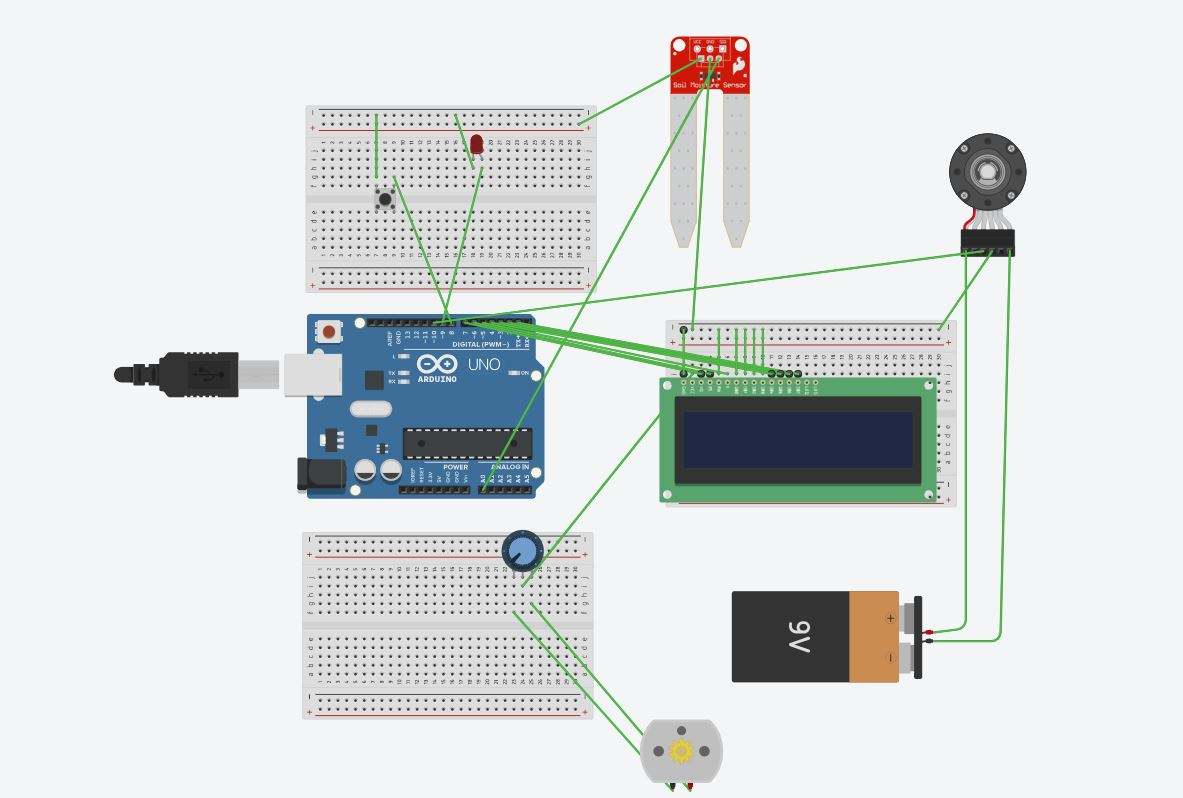
\includegraphics[width=1\linewidth]{Ciruit_Tinkercad.JPG}
    \caption{Circuit was first designed in Tinkercad for initial planning.}
\end{figure}
\begin{figure}
    \centering
    \includegraphics[width=1\linewidth]{Final_Circuit.jpg} % Add actual image file
    \caption{Final circuit setup implemented on a breadboard.}
\end{figure}

\section{Contributions}
The project was a collaborative effort, and the contributions of each member are as follows:
\begin{itemize}
    \item \textbf{Aidan Swan:} Lab write-up, documentation and  circuit building, and RTC code.
    \item \textbf{Nathan Saxe:} Fan motor, stepper motor, and water sensor code.
    \item      \textbf{Canon Leahy:} Schematic creation and my delay code.
    \item \textbf{Nate Gomez:} circuit building and temp / humidity code.

\end{itemize}
\section{GitHub Repository}
The full project, including code, documentation, and design files, can be found in the following GitHub repository:
\url{https://github.com/NathanSaxe/CPE301-Final-Project}

The repository contains:
\begin{itemize}
    \item Source code for the project.
    \item Video of it working.
    \item Datasheets used during its creation.

\end{itemize}

\end{document}
